\documentclass[12pt, twoside]{article} 
\newcommand{\hdir}{.}
\usepackage{./jmlda}
\usepackage[round]{natbib}
\usepackage{rotating}
\usepackage{tabularx} % for 'tabularx' env. and 'X' col. type
\setlength\extrarowheight{2pt} % make the tables look less cramped

\newtheorem{theorem}{Takkens(1981 Springer Lecture Notes in Mathematics vol 898, pp 366–81)}
\begin{document}
\title
	[поиск и восстановление зависимостей во временных рядах]
	{поиск и восстановление зависимостей во временных рядах}
\author
	[I. M. Latypov]
	{I. M. Latypov, E. Vladimirov, V. V. Strizhov}
\email
	{latypov.im@phystech.edu}
\organization	
	{MIPT}	
\abstract
	{
		При прогнозировании временных рядов, зависящих от других временных рядов, требуется решить задачу выявления связей между ними.
		Предполагается, что добавление связанных временных рядов в прогностическую модель повысит качество прогноза. В данной работе для
		обнаружения зависимостей между временными рядами предлагается совместить Convergent Cross Mapping с ODE-RNN. 
		}
\bigskip
\noindent

\maketitle
\textbf{Ключевые слова}: \emph{Neural CDE, CCM, временные ряды}

\section{Введение}
	Работа посвящена задаче поиска причинно-следственных связей между временными рядами.
	Эта задача актуальна, поскольку часто на практике приходится работать с многомерными временными рядами \citet{eural_ODE}, и учет зависимостей между координатами может улучшить качество предсказаний. 
		
		Существует множество методов для обнаружения связей между временными рядами. Среди них Тест Гренжера и метод сходящегося перекрестного отображения
	(convergent cross mapping, CCM) и другие. Идея работы CCM основана не теореме Таккенса (ссылка). Метод отображает временные ряды в траекторные многообразия и рассматривает зависимость траекторий эволюций этих рядов. Наша идея заключается в улучшении процесса построения отображения в траекторное многообразие. Для этого обучается модель ODE-RNN на эмбеддингах CCM алгоритма и скрытые состояния RNN слоев используются как новые эмбеддинги, и на них уже применяется метод CCM. 
		
		Преимуществом нашего метода перед CCM к тому же является возможность работать с рядами с нерегулярными наблюдениями.
	
	
\section{Связанные работы (related works)}
		
	
\section{Математическая постановка}
Обозначим $T = \{t_1, ... t_k\}$ - моменты наблюдений.

P.S. нужно будет перейти к вероятностной формулировке

$\mathbf{X} = [x_1, ... , x_k]^T$ - многомерный временной ряд, $x_i \in mathcal{R}^n$ - наблюдения $X$ в момент времени $t_i$.

Цель заключается в том, чтобы найти функцию(критерий) $F: \mathbb{R}^{n \times k } \rightarrow \mathbb R$, по значениям которой можно делать вывод о зависимостях между координатами временного ряда $X$.


\section{теоретические предпосылки}

Основой для построения метода послужила теорема Таккенса и метод CCM основанный на ней.

Пусть $M$ - компактное многообразие. Динамической системой $\phi$ c дискретным временем на $M$ назовем диффеоморфизм $\phi: M\rightarrow M$. В этом случае эволюция системы начинается с $x_0 \in M$ и следующие состояния определятся рекурсивно $x_{t+ 1} = \phi(x_t)$. 

Так же определим гладкую функцию $y: M \rightarrow \mathbb R$ - наблюдения за динамической системой. Хочется из набора наблюдений получить информацию об эволюции системы $\phi$ в $M$.

Для этого нам понадобится следующая теорема


\begin{theorem}
Пусть $M$ - компактное многообразие размерности $m$. Для пар $(\phi, y)$, где $\phi : M \rightarrow M$ гладкий диффеоморфизм и $y: M \rightarrow \mathbb R$ гладкая функция,
 общим свойством является то, что $\Phi: M \rightarrow \mathbb R^{2m + 1}$, определяемое как 

$$\Phi_{(\phi. y)} (x) = (y(x), y \circ \phi(x), ... , y \circ \phi^{2m}(x)) $$
является вложением $A(\phi) \rightarrow \mathbb R^{2m + 1}$. Под гладкостью понимается дважды непрерывная дифференцируемость.
\end{theorem}

$A(\phi)$ - аттрактор динамической системы.

То есть для изучения свойств траектории динамической системы $phi$ можно использовать траектории, которые получаются при этих погружениях.

Пусть даны две динамические системы: $\phi$ с наблюдениями $x$ на многообразии $M_x$ и $\psi$  c наблюдениями $y$ на многообразии $M_y$. 
Нужно выяснить, есть ли причинно-следственная связь между системами. Поскольку мы не имеем представления об устройстве многообразий рассмотрим их вложения $\Phi_(\phi, x)$ и $\Phi_(\psi, y)$.

(TODO   расписать здесь идею CCM) 

Мы хотим проверить, можно ли вместо таких погружений рассматривать систему $psi$, которая будет развиваться в зависимости от наблюдений за $\phi$. Более формально:

Есть динамическая система $\phi$, которая развивается в многообразии $M$ размерности $m$. $y: M \rightarrow \mathbb R$ - непрерывный наблюдатель за системой $\phi$.
Введем (динамическую сисему ?) $\psi: \mathbb R^{n + 1} \rightarrow \mathbb {R}$. Её вектора обозначим $\gamma$ так, что 

\begin{equation}
	\begin{split}
		\gamma_0 = f(y_0) \\ 
		\gamma_{k + 1} = \psi(\gamma_k, y_k)
    \end{split}
\end{equation}

Если динамическая система $\phi$ задана с непрерывным временем, то вместо функции $\psi$ рассмотрим интеграл

\begin{equation}
	\begin{split}
		\gamma(t_0) = f(y(t_0)) \\
		\gamma(t) = \int_{t_0}^{t} \psi(\gamma(\tau), y(\tau)) d\tau
    \end{split}
\end{equation}

Ввиду невозможности непрерывного измерения $y$ при интегрировании будем использовать интерполяцию или $ y(\tau) = g(\gamma(t))$ и уточнять y по мере интегрирования.



\section{Предлагаемый метод}
----------------------------------------------------------------------------

пока просто накидал идей

---------------------------------------------------------------------------

Для выявления зависимости рядов мы предлагаем использовать скрытые состояния нашей архитектуры как эмбеддинги в CCM. 

Предлагаемая архитектура является доработанным ODE-RNN. ODE-RNN обеспечивает непрерывную эволюцию скрытого состояния, но во время применения RNN эта непрерывность нарушается.
С целью исправления этого недостатка в интегратор подается сам RNN модуль, но тогда возникает проблема - неоткуда брать вход в RNN модуль. Эту проблему предлагается решить подачей на вход 
RNN модулю его же предсказания. Таким образом во время интегрирования модуль будет учиться порождать последовательность на которой обучается.

Чтобы при интегрировании не случался экспоненциальный рост значений ввиду собственных значений RNN модуля больше 1 применяется Batch Normalization


\begin{figure}[ht!]
	\centering
	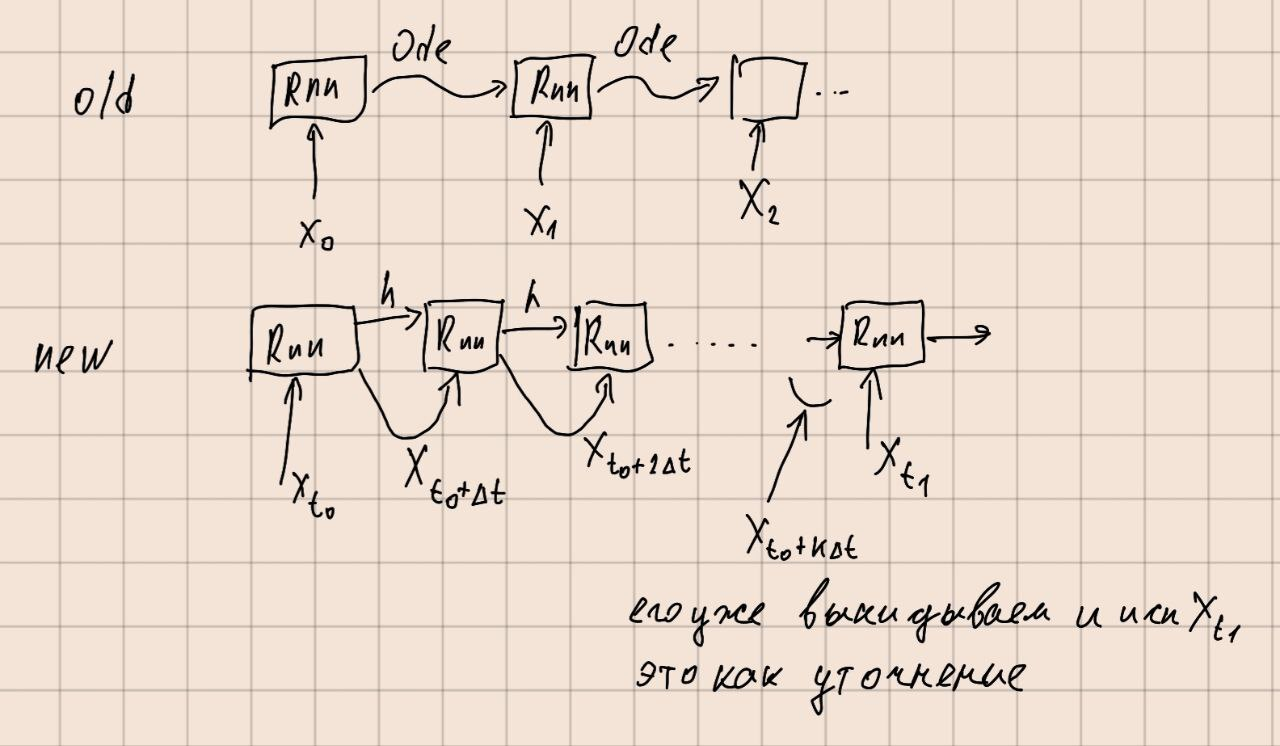
\includegraphics[width=90mm]{pic_1.jpg}
	\caption{A simple caption \label{overflow}}
\end{figure}

Fрхитектура обладает хорошей способностью к обучению, об этом в экспериментах  

Для выяснения зависимости рядов delay embedding ам сопоставляется скрытое состояние после пропускания его через сетку. После этого к полученным погружениям применяется CCM.

Так же выяснилось, что метод CCM не может работать с delay embedding ами при большом количестве наблюдений - корреляция (определенная в CCM) уходит с ноль при большом количестве точек наблюдения. 
Нащ метод не обладает таким недостатком.

Недостатком же метода является появление корреляции между независимыми временными рядами при большой размерности погружения. Мы предполагаем что это связано с проклятием размерности. 
Обычный CCM лишен такого недостатка. Для обхода недостатка достаточно размерность погружения сделать достаточно маленькой (например 2)



\section{эксперименты}
	Провели эксперименты, можно посмотреть на гите
	
\section{Теоритическое обоснование}
	
\section{Заключение}

\bibliographystyle{plain}
\bibliography{library.bib}

\newpage

\begingroup
\fontsize{8pt}{10pt}\selectfont
\begin{sidewaystable}
	\caption{сравнение методов}
		\begin{tabular}{|l|l|l|l|}
			\hline
			Метод            & краткое описание                                                                                                                                                                                                                                                                 & достоинства                                                                                                 & недостатки                                                                                                                                                                                                              \\ \hline
			Тест Гренжера    & \begin{tabular}[c]{@{}l@{}}Пусть $U, V$ - временные ряды. \\ $U$ предсказывают с  использованием \\ $V$ и без использования.При существенном\\  улучшении предсказаний делается вывод \\ о зависимости рядов.\end{tabular}                                                       & Легко применять                                                                                             & \begin{tabular}[c]{@{}l@{}}не дает представлений о виде \\ зависимости рядов. \\ К тому же предсказания могут не \\ улучшиться из-за неверной модели.\end{tabular}                                                      \\ \hline
			Кросс Корреляция & \begin{tabular}[c]{@{}l@{}}Проверяется корреляция  сдвинутых\\ по времени компонент временного ряда. \\ Критерием служит максимальная \\ полученная корреляция\end{tabular}                                                                                                      & Легко применять                                                                                             & \begin{tabular}[c]{@{}l@{}}Приходится использовать весь датасет\\  + квадратичное от длины ряда \\ время работы. Так же хорошо известно, \\ что корреляция не является достаточным \\ условием зависимости\end{tabular} \\ \hline
			CCM              & \begin{tabular}[c]{@{}l@{}}компоненты временного ряда отображаются \\ в траектороное  подпространство и\\  проверяется возможность отображения \\ одной траектории на другую.\\  Критерием зависимости служит значение \\ введенной в работе специальной корреляции\end{tabular} & \begin{tabular}[c]{@{}l@{}}Легко применять.\\  Работает лучше \\ методов предложенных \\ выше.\end{tabular} & \begin{tabular}[c]{@{}l@{}}использование всего датасета, \\ квадратичное от длины ряда время работы.\\  Так же ислледование \textbackslash{}citep\{CCM\_PA\} \\ выделяет другие недостатки.\end{tabular}                \\ \hline
			CMM + ODE-RNN    & обучаем сетку, применяем CCM                                                                                                                                                                                                                                                     & \begin{tabular}[c]{@{}l@{}}Точнее может выявлять \\ зависимости между \\ временными рядами\end{tabular}     & \begin{tabular}[c]{@{}l@{}}Нужно обучать на достаточно \\ \\ большом куске данных\end{tabular}                                                                                                                          \\ \hline
		\end{tabular}
	\end{sidewaystable} 
\endgroup
\end{document}